%%%%%%%%%%%%%%%%%%%%%%%%%%%%%%%%%%%%%%%%%%%%%%%%%%%%%%%%%%%%%%%%%%%%%%%%%%%%%%%
%
% Filename: ira-analysis.tex
% Author:   David Oniani
% Modified: November 17, 2019
%  _         _____   __  __
% | |    __ |_   _|__\ \/ /
% | |   / _` || |/ _ \\  /
% | |__| (_| || |  __//  \
% |_____\__,_||_|\___/_/\_\
%
%%%%%%%%%%%%%%%%%%%%%%%%%%%%%%%%%%%%%%%%%%%%%%%%%%%%%%%%%%%%%%%%%%%%%%%%%%%%%%%

%%%%%%%%%%%%%%%%%%%%%%%%%%%%%%%%%%%%%%%%%%%%%%%%%%%%%%%%%%%%%%%%%%%%%%%%%%%%%%%
% Document definition
%%%%%%%%%%%%%%%%%%%%%%%%%%%%%%%%%%%%%%%%%%%%%%%%%%%%%%%%%%%%%%%%%%%%%%%%%%%%%%%

\documentclass{article}

%%%%%%%%%%%%%%%%%%%%%%%%%%%%%%%%%%%%%%%%%%%%%%%%%%%%%%%%%%%%%%%%%%%%%%%%%%%%%%%
% Packages and related settings
%%%%%%%%%%%%%%%%%%%%%%%%%%%%%%%%%%%%%%%%%%%%%%%%%%%%%%%%%%%%%%%%%%%%%%%%%%%%%%%

% Global, document-wide settings
\usepackage[margin=1in]{geometry}
\usepackage[utf8]{inputenc}
\usepackage[english]{babel}

% Bibliography and references
\usepackage[backend=biber]{biblatex}
\addbibresource{references.bib}

% Other packages
\usepackage{booktabs}
\usepackage{fancyhdr}
\usepackage[hang,flushmargin]{footmisc}
\usepackage{hyperref}
\usepackage{mathtools}
\usepackage[cache=false]{minted}
\usepackage{subfig}

%%%%%%%%%%%%%%%%%%%%%%%%%%%%%%%%%%%%%%%%%%%%%%%%%%%%%%%%%%%%%%%%%%%%%%%%%%%%%%%
% Miscellaneous
%%%%%%%%%%%%%%%%%%%%%%%%%%%%%%%%%%%%%%%%%%%%%%%%%%%%%%%%%%%%%%%%%%%%%%%%%%%%%%%

% Setting stuff
\setlength{\parindent}{0pt}  % Remove indentations from paragraphs
\pagestyle{fancy}            % This allows to do fancy headers and footers
\fancyhf{}                   % No additional page numbering (or other stuff)
\cfoot{\thepage}             % Display page number at the bottom, in the center

% PDF information and nice-looking urls
\hypersetup{%
  pdfauthor={David Oniani},
  pdftitle={Textual and Statistical Analysis of Russian IRA Facebook Advertisements},
  pdfsubject={Statistics, Textual Analysis, Influence Campaign},
  pdfkeywords={Statistics, Textual, Influence, Campaign, Intelligence},
  pdflang={English},
  colorlinks=true,
  linkcolor={blue!50!black},
  citecolor={blue!50!black},
  urlcolor={blue!50!black}
}

% Put a centered header of a footnote size on the top of each page
\chead{\footnotesize{Textual and Statistical Analysis of Russian IRA Facebook
                     Advertisements}}

%%%%%%%%%%%%%%%%%%%%%%%%%%%%%%%%%%%%%%%%%%%%%%%%%%%%%%%%%%%%%%%%%%%%%%%%%%%%%%%
% Author(s), title, and date
%%%%%%%%%%%%%%%%%%%%%%%%%%%%%%%%%%%%%%%%%%%%%%%%%%%%%%%%%%%%%%%%%%%%%%%%%%%%%%%

% Author(s)
\author{David Oniani\\
        Luther College\\
        \href{mailto:oniada01@luther.edu}{oniada01@luther.edu}}

% Title
\title{\textbf{Textual and Statistical Analysis of Russian IRA Facebook Advertisements}\\
       \medskip
       \small \textsuperscript{*}The paper is written in the scope of a
       student-faculty collaborative\\ summer research with professor Richard
       K. Merritt (\href{mailto:merritri@luther.edu}{merritri@luther.edu}).}

% Date
\date{Last Revised: \today}

%%%%%%%%%%%%%%%%%%%%%%%%%%%%%%%%%%%%%%%%%%%%%%%%%%%%%%%%%%%%%%%%%%%%%%%%%%%%%%%
% Beginning of the document
%%%%%%%%%%%%%%%%%%%%%%%%%%%%%%%%%%%%%%%%%%%%%%%%%%%%%%%%%%%%%%%%%%%%%%%%%%%%%%%

\begin{document}
\maketitle

%%%%%%%%%%%%%%%%%%%%%%%%%%%%%%%%%%%%%%%%%%%%%%%%%%%%%%%%%%%%%%%%%%%%%%%%%%%%%%%
% Abstract
%%%%%%%%%%%%%%%%%%%%%%%%%%%%%%%%%%%%%%%%%%%%%%%%%%%%%%%%%%%%%%%%%%%%%%%%%%%%%%%

\begin{abstract}

\noindent The 2016 United States Presidential Election was targeted by an
unprecedented intelligence and influence campaign. Arising out of Russian
so-called Internet Research Agency (IRA), it sought to sow discord, attack
the fissures of the United States, and ultimately, sway the election results.
~\cite{ira2016}~\cite{ira2016data} In 2018, a portion of the IRA-backed
Facebook advertisements was released by The United States House Permanent
Select Committee on Intelligence. All of the advertisements are in the PDF
format. We have scraped the PDF files and present the results obtained by both
textual and statistical analysis of the above-mentioned data. Authorship
attribution and sentiment analysis were also performed.~\footnote{Please note
that the paper does not discuss the political implications of these actions,
but attempts to explore the methods of persuasion that were employed in this
influence campaign.}~\cite{ira2016csvdata} In addition, we have made the data
publicly available for other researchers and/or interested people in a much
nicer and easier-to-manipulate CSV format.

\end{abstract}

%%%%%%%%%%%%%%%%%%%%%%%%%%%%%%%%%%%%%%%%%%%%%%%%%%%%%%%%%%%%%%%%%%%%%%%%%%%%%%%
% Data and Preparation
%%%%%%%%%%%%%%%%%%%%%%%%%%%%%%%%%%%%%%%%%%%%%%%%%%%%%%%%%%%%%%%%%%%%%%%%%%%%%%%

\section{Data and Preparation}

The dataset was scraped from~\cite{ira2016data} more than 3,500 Russian IRA
Facebook~\footnote{In the paper, words ``advertisement'' and ``post'' are used
interchangeably.} posts made publicly available in the PDF format by the House
Intelligence Committee. We used a free and open-source \texttt{Python} library
~\cite{pdftotext} \texttt{pdftotext} to scrape the data. Many PDF files were
formatted in a way that it was virtually impossible for \texttt{pdftotext} to
parse them correctly. For this reason, we have manually reviewed most of the
CSV files for validity.~\cite{ira2016csvdata} All the CSV files have been made
publicly available. It is important to note that the dataset is just a sample
of a bigger dataset and, albeit \textit{less likely}, might not be a good
representation of the overall campaign.

\medskip

In total, there are 5 different sets of the datasets.
Figure 1 categorizes them.

\begin{figure}[H]
  \centering
  \begin{tabular}{*{5}{c}}
    \toprule
    Set & Dataset 1 & Dataset 2 & Dataset 3 & Dataset 4\\
    \midrule
    all  & all.csv & N/A & N/A & N/A\\
    \midrule
    by-year & year-2015.csv & year-2016.csv & year-2017.csv & N/A\\
    \midrule
    year-2015 & 2015-Quarter-2.csv & 2015-Quarter-3.csv & 2015-Quarter-4.csv & N/A\\
    \midrule
    year-2016 & 2016-Quarter-1.csv & 2016-Quarter-2.csv & 2016-Quarter-3.csv & 2016-Quarter-4.csv\\
    \midrule
    year-2017 & 2017-Quarter-1.csv & 2017-Quarter-2-April.csv & 2017-Quarter-2-May.csv & 2017-Quarter-3.csv\\
    \bottomrule
  \end{tabular}
  \caption{Categorization of the Sets of the Datasets}
\end{figure}

All datasets are of the same ``shape.'' Below is the output of Python's pandas
package command \mintinline{python}{dataset.dtypes}.

\begin{figure}[H]
  \begin{minted}[fontsize=\normalsize]{python}
    import pandas as pd

    data = pd.read_csv("./data/csv/all/all.csv", na_filter=False, thousands=",")
    print(data.dtypes)

    Ad ID                      int64
    Ad Text                   object
    Ad Landing Page           object
    Ad Targeting Location     object
    Excluded Connections      object
    Age                       object
    Language                  object
    Placements                object
    People Who Match          object
    Friends of Connections    object
    Ad Impressions             int64
    Ad Clicks                  int64
    Ad Spend                  object
    Ad Creation Date          object
    Ad End Date               object
    dtype: object
  \end{minted}
  \caption{Dataset Layout}
\end{figure}

Every row represents a Facebook advertisement which has 15 different properties
and thus, the dataset has 15 columns. Out of these columns, only 3 are integer
values, namely ``Ad ID'', ``Ad Impressions'', and ``Ad Clicks.'' The rest of
the columns are of the string type. This is the case for all datasets.

%%%%%%%%%%%%%%%%%%%%%%%%%%%%%%%%%%%%%%%%%%%%%%%%%%%%%%%%%%%%%%%%%%%%%%%%%%%%%%%
% Common Words
%%%%%%%%%%%%%%%%%%%%%%%%%%%%%%%%%%%%%%%%%%%%%%%%%%%%%%%%%%%%%%%%%%%%%%%%%%%%%%%

\section{Word Analysis}

Among the strategies utilized by this influence campaign, one that stood out
the most was the exploitation of internal issues of the United States by
leveraging the social, political, and historical backgrounds of the country.

\medskip

The word choice played a crucial role in the effectiveness of the influence
campaign. An overwhelming number of advertisements referenced issues including
race, police, immigration, religion, and guns. Figure 2 shows a bar chart with
TOP 25 most commonly used words after eliminating linking verbs, prepositions,
pronouns, and other
~\footnote{The list of all eliminated words is provided at\\
\url{https://github.com/oniani/ira-analysis/blob/master/eliminated-words.txt}.}
non-relevant words.

\begin{figure}[H]
\centering
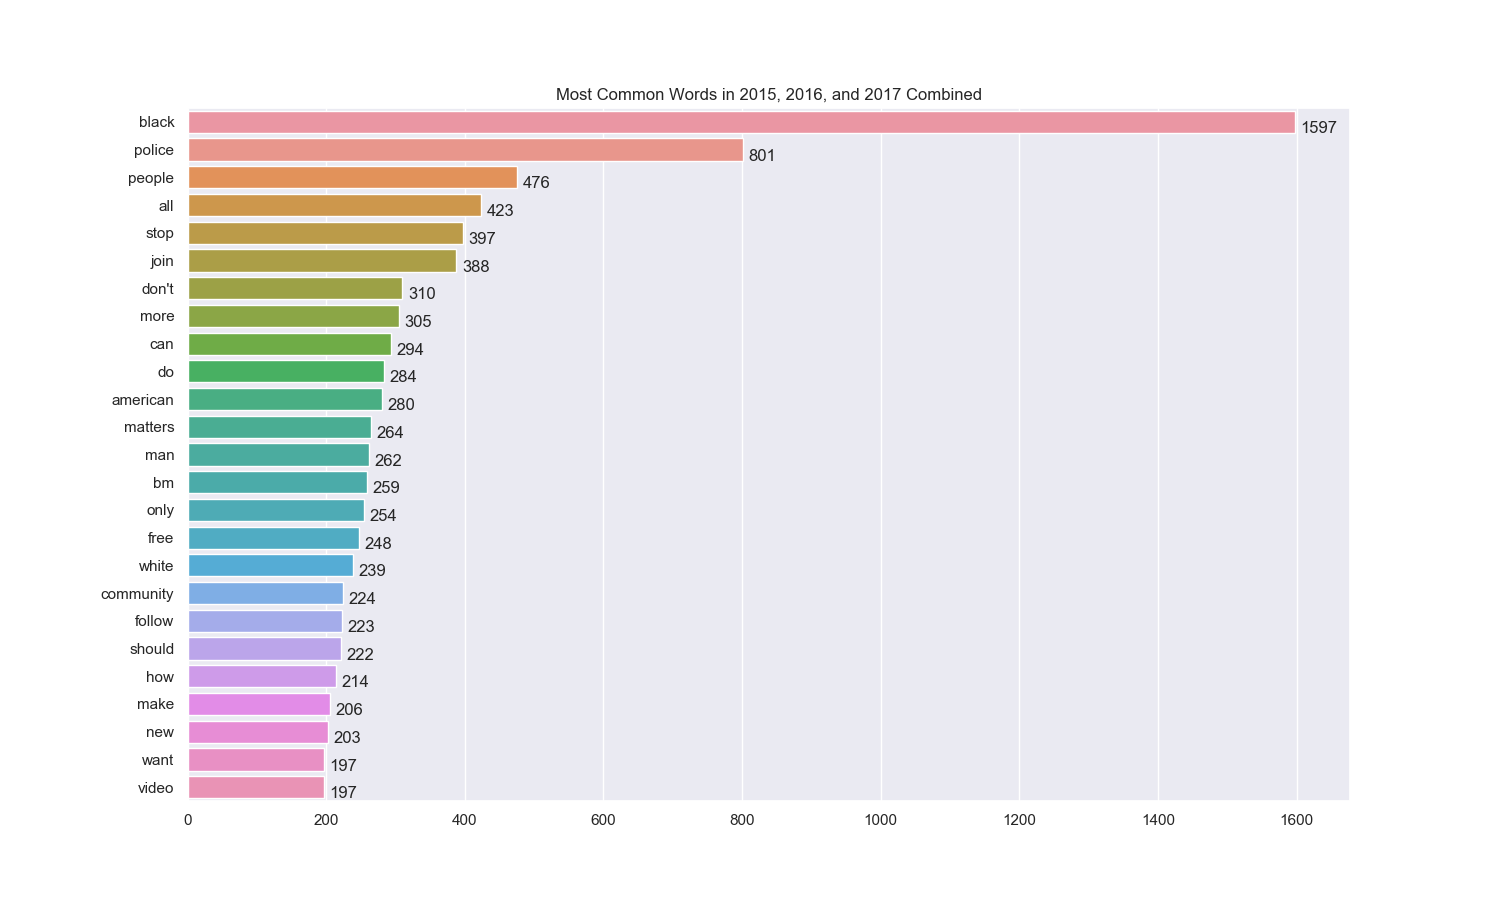
\includegraphics[width=\linewidth]{./image/barchart-plots/barchart_word_counts.png}
\caption{Most common words in 2015, 2016, and 2017 combined.}
\end{figure}

The vast majority of Facebook ads featured words and phrases related to race
and race-based discrimination. More than 50\% of the posts referenced race and
generated over 25 million ad impressions. Three most commonly used words were
``black'', ``police'', and ``people.''

\medskip

Words associated with ``taking action'' such as ``join'', ``stop'', ``do'',
``follow'' etc.~were used extensively for persuasive purposes. These words in
conjunction with others such as ``American'', ``matters'', ``community'' etc.
further increased the persuasive quality of advertisements by metaphorically
connecting them with cultural and social identities of people and fueling
hateful rhetoric.

\medskip

117 posts referenced words ``Clinton'' and ``Trump'' (last names of the
presidential candidates at the time) accounting for 61,774 ad clicks and
853,855 ad impressions in total. There were 3 posts mentioning word ``Donald''
and not mentioning ``Trump'' resulting in 226 clicks and 2,182 impressions, but
none mentioning ``Hilary'' and not ``Clinton.''

\medskip

There was only a single ad directly referencing Russia with 135 clicks and
1,236 impressions. The advertisement was denouncing the request for the
increase in the US military spendings and making a comparison with the Russian
military budget.

%%%%%%%%%%%%%%%%%%%%%%%%%%%%%%%%%%%%%%%%%%%%%%%%%%%%%%%%%%%%%%%%%%%%%%%%%%%%%%%
% Sentiment Analysis
%%%%%%%%%%%%%%%%%%%%%%%%%%%%%%%%%%%%%%%%%%%%%%%%%%%%%%%%%%%%%%%%%%%%%%%%%%%%%%%

\section{Sentiment Analysis}

For sentiment analysis, we used a free and open-source \texttt{Python} library
\texttt{TextBlob}. Interestingly, out of all Facebook posts with a non-empty
\texttt{Ad Text} value, 1643 were positive, 900 negative, and 932 neutral
leaving the overall tone of the posts positive. Yet, the claim is not strong
or significant as the polarity levels were always near zero. Such low polarity
levels, however, demonstrate a highly intelligent design of advertisements.

\medskip

As the \texttt{Ad Text}s did not give us any strong evidences, we looked at the
negativity levels across all three years and found a consistent trend (Figure 4).

\begin{figure}[H]
  \centering
  \begin{tabular}{*{5}{c}}
    \toprule
    Subjectivity & Year 2015 & Year 2016 & Year 2017 & 2016 (\%)\\
    \midrule
    1.0  & 154 & 562 & 176 & 63.004\\
    \midrule
    0.75 & 150 & 547 & 169 & 63.164\\
    \midrule
    0.5  & 123 & 405 & 120 & 62.500\\
    \midrule
    0.25 & 15 & 81 & 22 & 68.644\\
    \midrule
    0.15 & 5 & 33 & 10 & 68.750\\
    \midrule
    0.1  & 2 & 11 & 6 & 57.895\\
    \midrule
    0.05 & 1 & 5 & 2 & 62.500\\
    \bottomrule
  \end{tabular}
  \caption{Analyzing Negativity}
\end{figure}

Notice that for any given year and at any subjectivity level, year 2016
consistently comprises around 60\% of all posts. The sudden change in strategy
and increased levels of negativity could be linked to approaching Presidential
Election and making people take an action by voting for candidates promoted by
these ads. The year of the Presidential Election was rather negative.

%%%%%%%%%%%%%%%%%%%%%%%%%%%%%%%%%%%%%%%%%%%%%%%%%%%%%%%%%%%%%%%%%%%%%%%%%%%%%%%
% Authorship Attribution
%%%%%%%%%%%%%%%%%%%%%%%%%%%%%%%%%%%%%%%%%%%%%%%%%%%%%%%%%%%%%%%%%%%%%%%%%%%%%%%

\section{Authorship Attribution}

Since all of these posts were issued by the same organization/entity, it was
interesting to see if there are some common patterns between the Facebook ads
of 2015, 2016, and 2017. For this reason, we have performed authorship
attribution tests by implementing~\cite{koppel11} the paper by Koppel et.~al.

\medskip

We have performed 3 authorship attribution tests:

\begin{enumerate}
  \item Assume that the Facebook ads of years 2016 and 2017 were written by the
        same author and assess the similarity for the ads of the year 2015.

  \item Assume that the Facebook ads of years 2015 and 2017 were written by the
        same author and assess the similarity for the ads of the year 2016.

  \item Assume that the Facebook ads of years 2015 and 2016 were written by the
        same author and assess the similarity for the ads of the year 2017.
\end{enumerate}

In all three cases, we had to merge different posts to meet the required
minimum text length of 500 words.~\footnote{Note that because of randomization,
texts were somewhat scrambled and are not available in any format. That said,
one can easily redo the authorship attribution with similar accuracy using the
algorithm which is already implemented and resides in the GitHub repository,
\url{https://github.com/oniani/ira-analysis/tree/master/koppel11}.} This was
done using randomization to avoid bias.~\footnote{Results JSON:
\url{https://github.com/oniani/ira-analysis/tree/master/koppel11/results}}
Results are available in the form of JSON files formatted in the manner shown
below.

\begin{figure}[H]
  \begin{minted}[frame=single,tabsize=2,fontsize=\normalsize]{js}
  {
    "answers": [
      {
        "unknown_text": "2015-unknown1.txt",
        "author": "candidate2016",
        "score": 0.58
      },
      ...
      {
        "unknown_text": "2015-unknown56.txt",
        "author": "candidate2016",
        "score": 0.76
      }
    ]
  }
  \end{minted}
  \caption{JSON example}
\end{figure}

The first answer tells us that the unknown text was written in year 2015, and
that there is 58\% chance that it was written by the author of Facebook ads of
year 2016. The last answer shows that there is 76\% chance that the given ad,
which was posted in 2015, was authored by the entity who wrote the posts in
year 2016.

\medskip

Figure 6 shows the results obtained after performing all three above-mentioned
authorship attribution tests.

\begin{figure}[H]
  \centering
  \begin{tabular}{*{2}{c}}
    \toprule
    Years & Similarity (\%)\\
    \midrule
    2016 and 2017 & 72.509 (similarity to 2015)\\
    \midrule
    2015 and 2017 & 68.516 (similarity to 2016)\\
    \midrule
    2015 and 2016 & 62.392 (similarity to 2017)\\
    \midrule
    Average (2015, 2016, and 2017) & 67.806\%\\
    \bottomrule
  \end{tabular}
  \caption{Average Similarity}
\end{figure}

On average, there is approximately 68\% similarity across texts suggesting that
the design strategy for these posts were roughly similar.

%%%%%%%%%%%%%%%%%%%%%%%%%%%%%%%%%%%%%%%%%%%%%%%%%%%%%%%%%%%%%%%%%%%%%%%%%%%%%%%
% General Statistics
%%%%%%%%%%%%%%%%%%%%%%%%%%%%%%%%%%%%%%%%%%%%%%%%%%%%%%%%%%%%%%%%%%%%%%%%%%%%%%%

\section{General Statistics}

The distribution of posts across all three years is of a bimodal nature with
two peaks in quarters 2 and 4 of the year 2016. Given the fact that the US
Presidential Election was held in the fourth quarter of 2016, it is surprising
that the number of posts in the second quarter exceeded that of the fourth
quarter.

\begin{figure}[H]
\centering
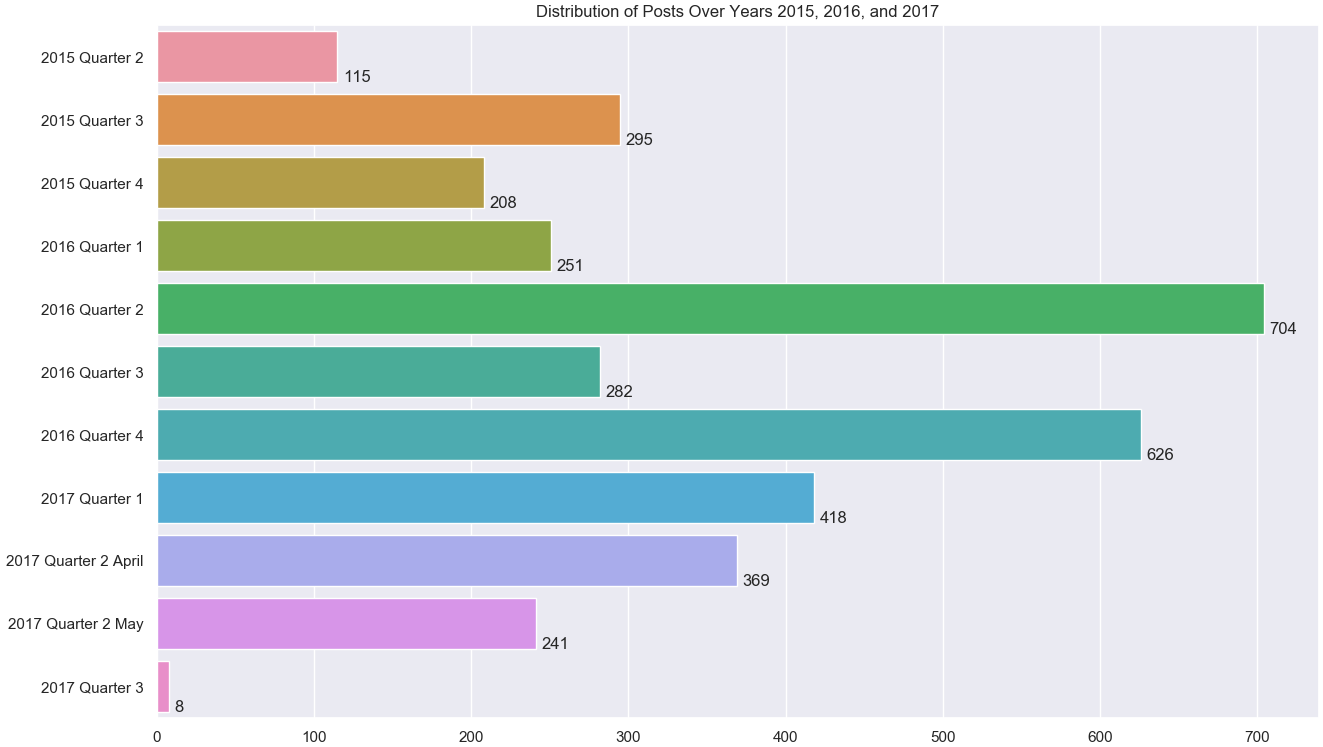
\includegraphics[width=\linewidth]{./image/barchart-plots/barchart_distribution_of_posts.png}
\caption{Distribution of Posts Over Years 2015, 2016, and 2017.}
\end{figure}

As for ad spendings, the fourth quarter of 2016 exceeds that of any quarter,
with the second quarter coming next. Interestingly, most of the ads were paid
in the Russian currency (ruble) with two exceptions (4 posts in total) in 2016
quarter 3 and 2017 quarter 1 when IRA spent \$74.000 and \$35.330 respectively.

\begin{figure}[H]
\centering
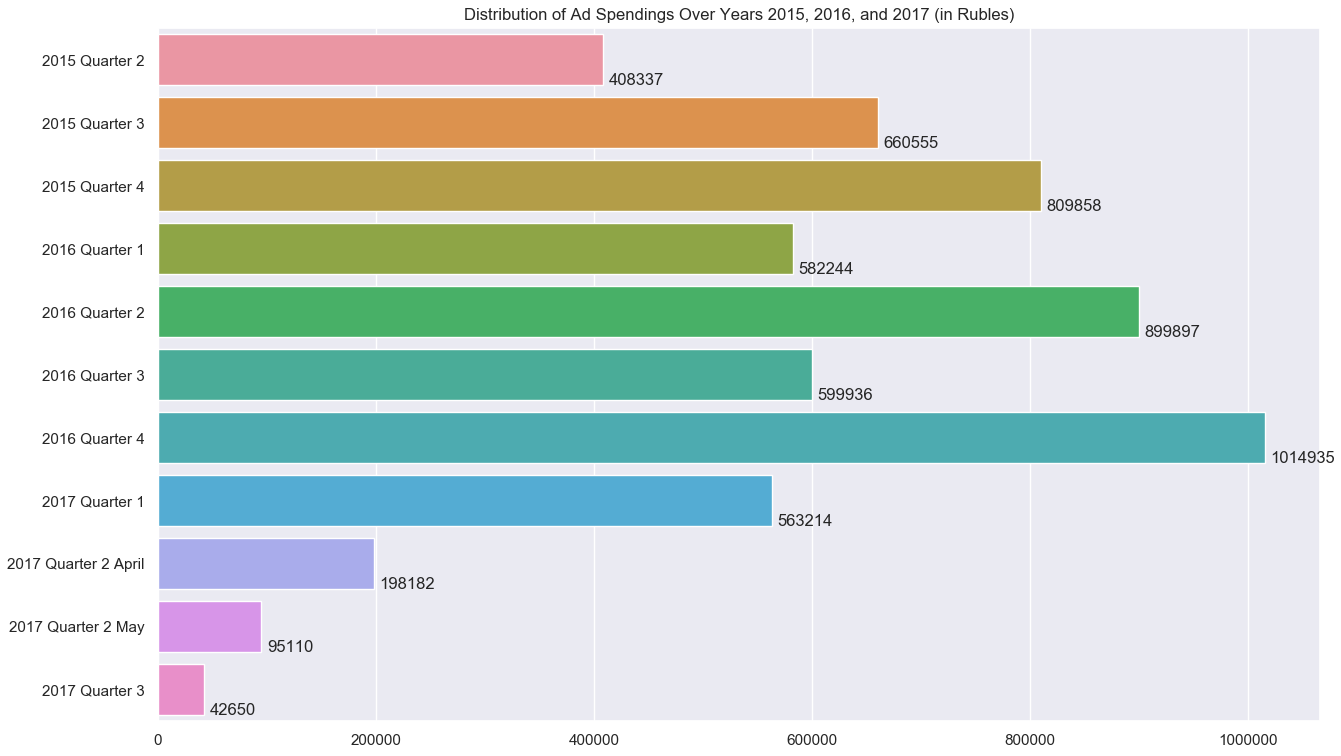
\includegraphics[width=\linewidth]{./image/barchart-plots/barchart_ad_spend_RU_distribution.png}
\caption{Distribution of Ad Spendings Over Years 2015, 2016, and 2017 (in rubles).}
\end{figure}

Furthermore, 99.8\% of all \textit{paid} ads across all three years were paid
in rubles. Figure 9 shows a chart with the number of posts based on currency.

\begin{figure}[H]
  \centering
  \begin{tabular}{*{2}{c}}
    \toprule
    Currency & \text{Total (All Years)}\\
    \midrule
    RUB & 2549\\
    \midrule
    USD & 5\\
    \midrule
    \footnotemark~None & 787\\
    \midrule
    0 & 176\\
    \bottomrule
  \end{tabular}
  \caption{Number of Posts Depending on the Currency.}
\end{figure}
~\footnotetext{None values can be considered 0.}

As the information for the reader, the Russian ruble is used only in Russia,
Belarus, and two regions of Georgia, which are considered by Russia as
partially recognized states of Abkhazia and South Ossetia.

\medskip

IRA was somewhat liberal toward age, with 69.542\% of advertisements targeting
all individuals of age 18 or more. Figure 10 shows the distribution of these ads.

\begin{figure}[H]
\centering
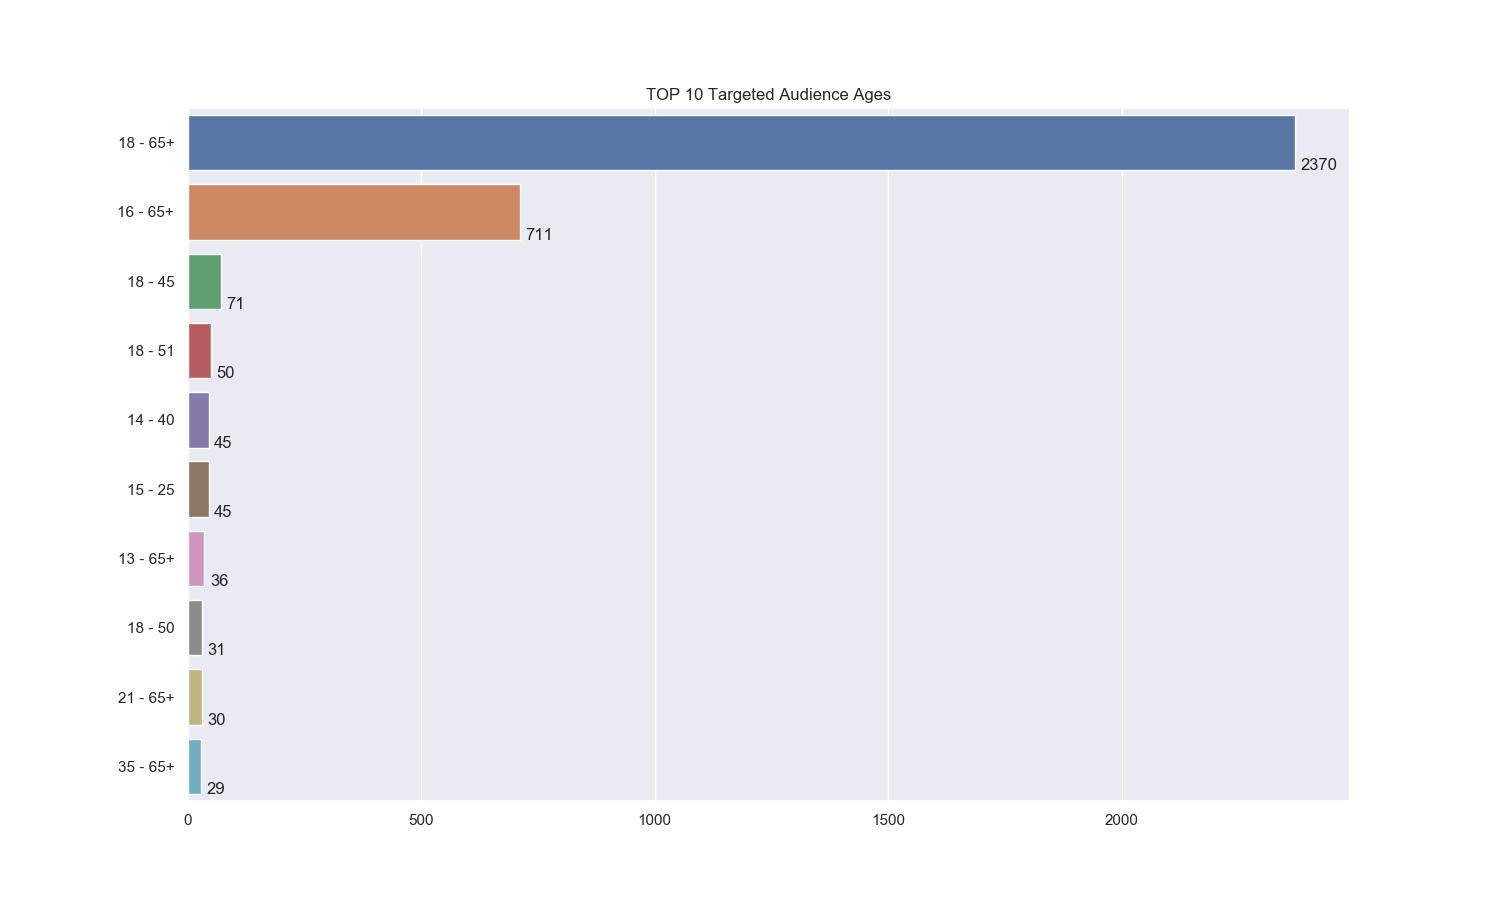
\includegraphics[width=\linewidth]{./image/barchart-plots/barchart_targeted_age.png}
\caption{Distribution of Posts Based on Age (Years 2015, 2016, and 2017).}
\end{figure}

Surprisingly, nearly all advertisements that targeted the 15 -- 25 age category
featured a website \url{musicfb.info} which~\cite{musicfb-info} appears to be
link to a Chrome extension (currently unavailable) and was registered in Saint
Petersburg, Russia (location of IRA). This is a notable fact since music is
strongly linked to emotions and can be used as a powerful weapon of
manipulation.

%%%%%%%%%%%%%%%%%%%%%%%%%%%%%%%%%%%%%%%%%%%%%%%%%%%%%%%%%%%%%%%%%%%%%%%%%%%%%%%
% Regression Analysis
%%%%%%%%%%%%%%%%%%%%%%%%%%%%%%%%%%%%%%%%%%%%%%%%%%%%%%%%%%%%%%%%%%%%%%%%%%%%%%%

\section{Regression Analysis}

We would like to determine if there is a statistically significant relationship
between two quantitative variables: the textual length of an advertisement and
money spent on it. Finding the relationship between these variables will give
us an idea if there was some kind of priority attached to posts, depending on
the textual length.

\medskip

For this task, we use a linear regression approach. Note that we perform the
analysis only on the ads paid in rubles, the primary reason being not having
enough data points for USD (only 5 values).

\begin{figure}[H]
  \centering
  \subfloat[Money Spent VS Ad Spend Length]{{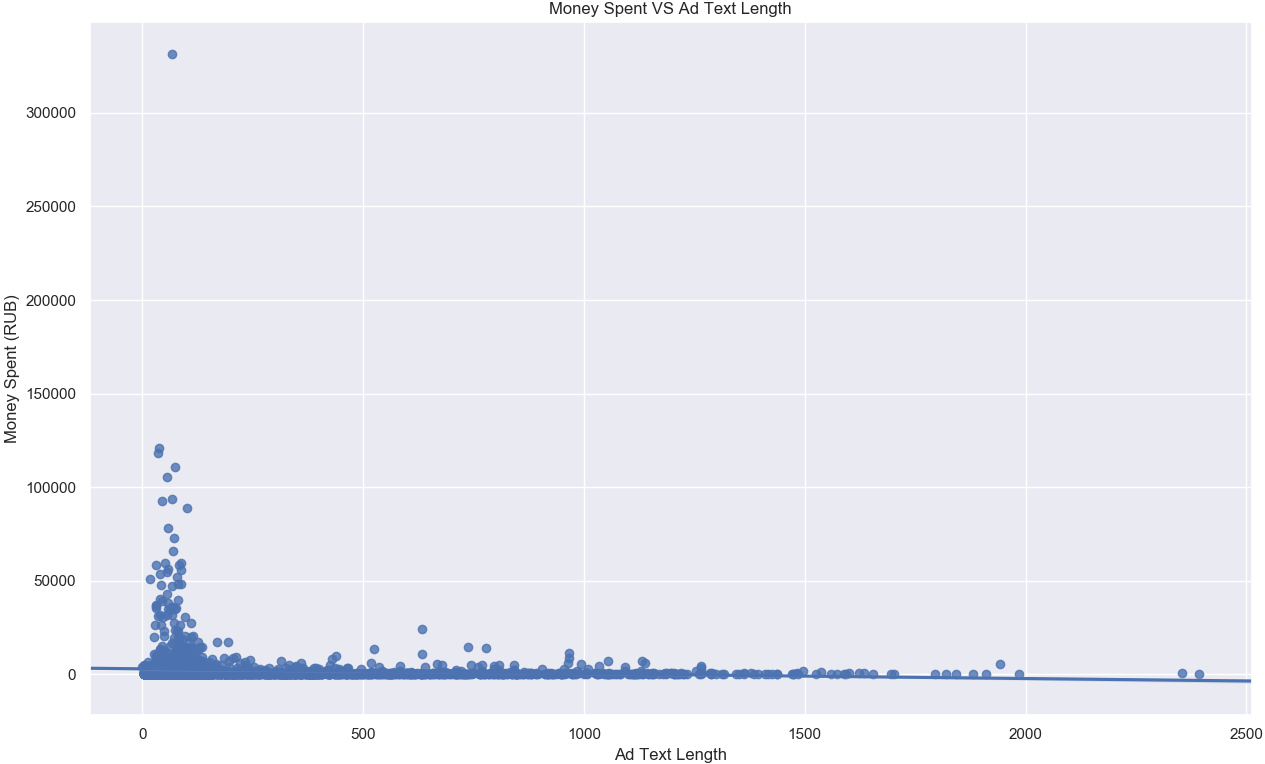
\includegraphics[width=0.5\linewidth]{./image/regression-plots/ad_spend_text_length_regression.png}}}
  \hfill
  \subfloat[Log Money Spent VS Log Ad Spend Length]{{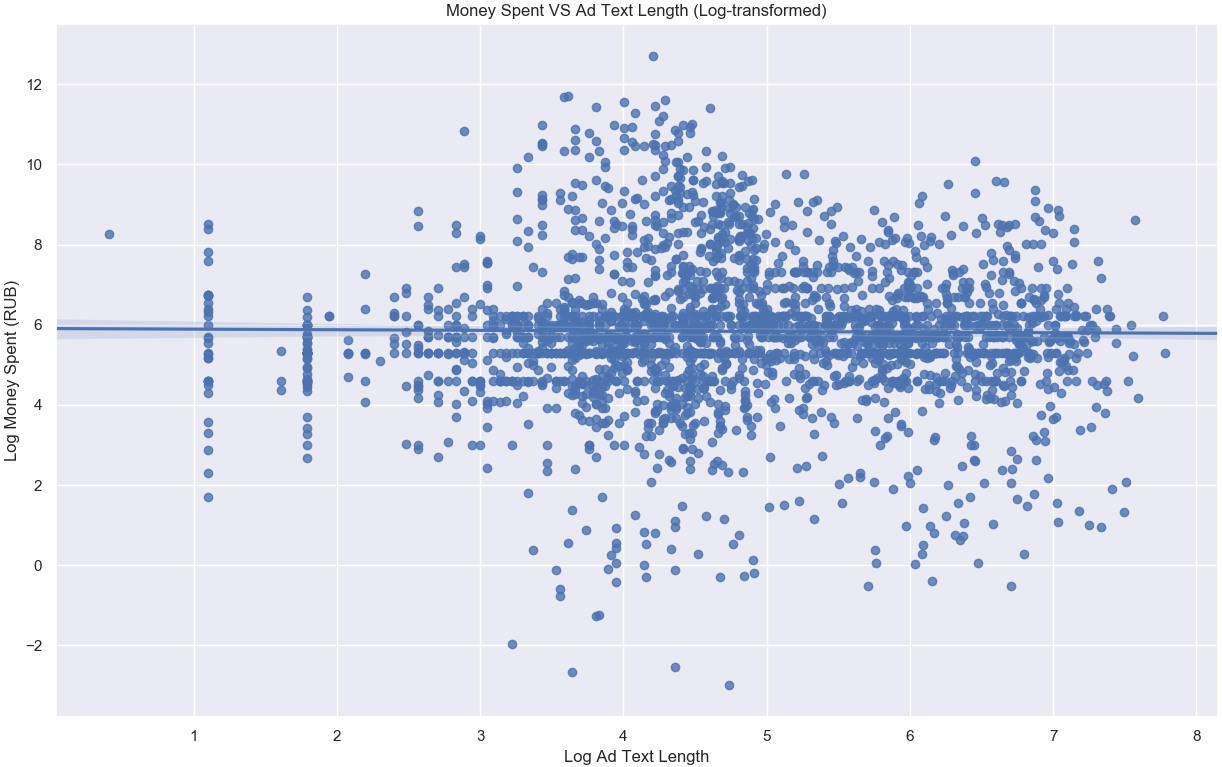
\includegraphics[width=0.5\linewidth]{./image/regression-plots/ad_spend_text_length_regression_log_transform.png}}}
  \caption{Simple VS Log-transformed}
\end{figure}

The first plot showed no strong relationship between the response and the
predictor. That said, the shape of the plot hinted us to apply the log
transformation. The log transformation, once again, verified our assumption
of no relationship. The numerical data in Figure 11 further reinforces our
observations.

\begin{figure}[H]
  \centering
  \begin{tabular}{*{2}{c}}
    \toprule
    \multicolumn{2}{c}{RUB (Without Log Transform)}\\
    \midrule
    Slope          & -2.594\\
    \midrule
    Intercept      & 2980.780\\
    \midrule
    R-squared      & 0.007\\
    \midrule
    P-value        & $3.680 * 10^{-5}$\\
    \midrule
    Standard Error & 0.627\\
    \bottomrule
  \end{tabular}
  \quad
  \begin{tabular}{*{2}{c}}
    \toprule
    \multicolumn{2}{c}{RUB (With Log Transform)}\\
    \midrule
    Slope          & -0.015\\
    \midrule
    Intercept      & 5.904\\
    \midrule
    R-squared      & 0.0001\\
    \midrule
    P-value        & $0.594 * 10^{-5}$\\
    \midrule
    Standard Error & 0.028\\
    \bottomrule
  \end{tabular}
  \caption{Linear Regression Analysis Results.}
\end{figure}

The chart above, R-squared equals 0.007, which tells us that only 0.7\%
of the variation in the money paid for advertisements is explained by the
number of characters. The residual standard error is 0.627 which is very small
compared to the intercept whose value is 2980.780 (RUB). The p-value equals
$3.680 * 10^{-5}$ which is a lot smaller than $0.05$ and makes the conclusion
statistically significant.

\medskip

Even after performing a log transformation, the results show no evidence of a
strong or even a weak relationship between the variables. The p-value reassures
us that the results are statistically significant.

\medskip

Although having no relationship is usually not the desired result, in our case,
we can conclude that posts were designed with no noticeable priorities
depending on the number of words in the ad text section.

%%%%%%%%%%%%%%%%%%%%%%%%%%%%%%%%%%%%%%%%%%%%%%%%%%%%%%%%%%%%%%%%%%%%%%%%%%%%%%%
% Binary Classifier
%%%%%%%%%%%%%%%%%%%%%%%%%%%%%%%%%%%%%%%%%%%%%%%%%%%%%%%%%%%%%%%%%%%%%%%%%%%%%%%

\section{Binary Classifier}

For the text classification purposes, we have built a binary classifier. The
program can, with the high accuracy, tell apart IRA and non-IRA texts. Model
has three features: text length, number of punctuation marks, and the frequency
of TOP 25 most common words discussed previously in the paper. We took the
ensemble learning approach and utilized the random forest classifier
(\texttt{RandomForestClassifier}) from the \textit{Scikit-learn} package with
180 estimators and unlimited depth. The non-IRA text for the separate label was
obtained from the \texttt{textgen} package
(\url{https://github.com/minimaxir/textgenrnn}). Figure 13 shows the measures
of robustness of the model.

\begin{figure}[H]
  \centering
  \begin{tabular}{*{2}{c}}
    \toprule
    Criterion & Value (\%)\\
    \midrule
    Precision & 97.2\%\\
    \midrule
    Recall    & 95.3\%\\
    \midrule
    Accuracy  & 96.2\%\\
    \bottomrule
  \end{tabular}
  \caption{Precision, recall, and accuracy of the model}
\end{figure}

Besides, we have provided a simple interface for the classification of the
textual data. The program is called \texttt{predict.py} and is available at
\url{https://github.com/oniani/ira-analysis/blob/master/nlp-model}.

%%%%%%%%%%%%%%%%%%%%%%%%%%%%%%%%%%%%%%%%%%%%%%%%%%%%%%%%%%%%%%%%%%%%%%%%%%%%%%%
% Conclusions
%%%%%%%%%%%%%%%%%%%%%%%%%%%%%%%%%%%%%%%%%%%%%%%%%%%%%%%%%%%%%%%%%%%%%%%%%%%%%%%

\section{Conclusions}

We have scraped PDF files made publicly available by The United States House
Permanent Select Committee on Intelligence and performed several different
analyses including textual and statistical. The obtained results gave us
important insights into a variety of different approaches and strategies used
in this influence campaign. We have also built a binary classifier for telling
apart IRA and non-IRA texts. We conclude that the advertisements were designed
in a complex and intelligent manner, targeting minorities, promoting hateful
rhetoric, and attempting to sway the election results. Much could be analyzed
and inferred from the provided datasets and any researcher and/or interested
person is free to use them for their research.

%%%%%%%%%%%%%%%%%%%%%%%%%%%%%%%%%%%%%%%%%%%%%%%%%%%%%%%%%%%%%%%%%%%%%%%%%%%%%%%
% References
%%%%%%%%%%%%%%%%%%%%%%%%%%%%%%%%%%%%%%%%%%%%%%%%%%%%%%%%%%%%%%%%%%%%%%%%%%%%%%%

\printbibliography

%%%%%%%%%%%%%%%%%%%%%%%%%%%%%%%%%%%%%%%%%%%%%%%%%%%%%%%%%%%%%%%%%%%%%%%%%%%%%%%
% The end of the document
%%%%%%%%%%%%%%%%%%%%%%%%%%%%%%%%%%%%%%%%%%%%%%%%%%%%%%%%%%%%%%%%%%%%%%%%%%%%%%%

\end{document}
